\documentclass[conference]{IEEEtran}
\usepackage{cite}
\usepackage{amsmath,amssymb,amsfonts}
\usepackage{graphicx}
\usepackage{textcomp}
\usepackage{booktabs}
\usepackage{multirow}
\usepackage{float}
\usepackage{placeins}
\usepackage{hyperref}
\usepackage{xcolor}
\usepackage{listings}
\usepackage{tabularx}
\usepackage{array}
\usepackage{algorithm}
\usepackage{algpseudocode}
\usepackage{makecell}

\definecolor{codegreen}{rgb}{0,0.6,0}
\definecolor{codepurple}{rgb}{0.58,0,0.82}

\lstset{
    basicstyle=\footnotesize\ttfamily,
    commentstyle=\color{codegreen},
    keywordstyle=\color{codepurple},
    stringstyle=\color{blue},
    frame=single,
    breaklines=true,
    columns=fullflexible,
    xleftmargin=2pt,
    xrightmargin=2pt
}

\correctBAPCfalse
\hyphenation{block-chain at-tes-ta-tion fed-er-at-ed learn-ing qua-ran-tine By-zan-tine}

\newcommand{\R}{\mathbb{R}}
\newcommand{\N}{\mathbb{N}}
\newcommand{\B}{\mathcal{B}}
\newcommand{\M}{\mathcal{M}}

\begin{document}

\title{Resilient Federated Learning: A Lightweight Snapshot-Based Rollback and\\Blockchain Attestation Framework\\Against Data Poisoning}

\author{\IEEEauthorblockN{Anonymous Authors}
\IEEEauthorblockANot applicable — under review}}

\maketitle

\begin{abstract}
Federated Learning (FL) enables collaborative model training across decentralized clients without sharing raw data, but remains highly vulnerable to data poisoning attacks where malicious clients submit corrupted updates. Existing defenses such as Byzantine-robust aggregation and anomaly detection impose significant computational overhead or fail against adaptive adversaries. This paper presents \textbf{RFL-Block}, a lightweight framework combining snapshot-based rollback recovery with a simplified blockchain attestation ledger for tamper-evident model versioning. Through extensive experiments on CIFAR-10 with a FedAvg topology of 10 clients (6 benign, 4 malicious), we demonstrate that snapshot rollback alone is fundamentally insufficient against persistent gradient inversion attacks, cycling indefinitely without recovery (0\% repair rate across 25 detection events). We identify client quarantine as the critical missing component and prove that a single rollback followed by permanent malicious client exclusion achieves full accuracy recovery ($60.36\%$ best vs. $63.29\%$ clean baseline, gap $= 2.93\%$) within one round of post-quarantine training. The framework adds only $15$--$45$ ms synthetic consensus delay per recovery event and requires no modifications to the underlying FL aggregation protocol. Our findings establish a general principle: in self-healing FL systems, \emph{detection is necessary but insufficient without exclusion}.
\end{abstract}

\begin{IEEEkeywords}
Federated Learning, data poisoning, self-healing, rollback recovery, blockchain attestation, client quarantine, gradient inversion attack
\end{IEEEkeywords}

\section{Introduction}
\label{sec:introduction}

Federated Learning (FL), introduced by McMahan et al.~\cite{mcmahan2017fl}, has established itself as a foundational paradigm for privacy-preserving distributed machine learning. In the canonical FL workflow, a central aggregation server coordinates $n$ clients, each holding a private dataset $\mathcal{D}_i$. At communication round $r$, the server broadcasts the current global model parameters $\theta^{(r)}$ to all clients. Each client performs $E$ local epochs of stochastic gradient descent on $\mathcal{D}_i$, producing an updated local model $\theta_i^{(r)}$. The server aggregates these updates via Federated Averaging (FedAvg)~\cite{mcmahan2017fl}:

\begin{equation}
\theta^{(r+1)} = \sum_{i=1}^{n} \frac{|\mathcal{D}_i|}{\sum_{j=1}^{n} |\mathcal{D}_j|} \cdot \theta_i^{(r)}
\label{eq:fedavg}
\end{equation}

\subsection{Motivation}
Despite its privacy-preserving design, FL introduces a fundamentally enlarged attack surface. Because the server cannot inspect raw client data, malicious participants can submit corrupted model updates designed to degrade global performance or implant hidden backdoors~\cite{bagdasaryan2020backdoor, bhagoji2019poisoning}. Data poisoning attacks exploit the collaborative nature of FL: even a minority of adversarial clients can disproportionately influence the aggregated model through gradient amplification or label flipping.

The research community has responded with three main defense paradigms:
\begin{enumerate}
    \item \textbf{Byzantine-robust aggregation} (Krum~\cite{blanchard2017krum}, Trimmed Mean~\cite{yin2018trimmed}, Median~\cite{yin2018trimmed}) that suppresses outlier updates through robust statistics.
    \item \textbf{Anomaly detection} methods~\cite{li2020flguard, tolanietal2020} that identify suspicious weight updates via dimensionality reduction or layer-wise distance metrics.
    \item \textbf{Blockchain-based attestation} frameworks~\cite{ramanan2022blockchainfl, majeed2021blockchainfl} that record model hashes on distributed ledgers for tamper-evident audit trails.
\end{enumerate}

However, existing approaches face fundamental limitations. Byzantine-robust aggregation incurs quadratic computational complexity in the number of clients for certain methods (e.g., Krum requires pairwise distance computation) and discards potentially useful update information. Anomaly detectors suffer from high false-positive rates under non-IID data distributions, where benign client updates naturally diverge. Full blockchain integration imposes prohibitive transaction fees ($\sim\$5$--$50$ per write on Ethereum) and block confirmation latency (12--15 seconds) that is incompatible with high-frequency FL rounds.

\subsection{Our Contributions}
This paper proposes \textbf{RFL-Block} (Resilient Federated Learning with Blockchain Attestation), a lightweight framework that achieves provable recovery against data poisoning attacks through three complementary mechanisms:

\begin{enumerate}
    \item \textbf{Snapshot-based rollback recovery} with real-time accuracy monitoring and automatic weight restoration upon poisoning detection. Every round's global model is persisted as a parameter snapshot, and the system continuously tracks the best observed accuracy.
    \item \textbf{A blockchain-style attestation ledger} implementing SHA-256 hash chaining across model snapshots. Each snapshot's hash is concatenated with the previous block's hash to form an immutable chain, enabling post-hoc forensic verification without smart contract costs.
    \item \textbf{A client quarantine protocol} that permanently excludes detected malicious clients from future training rounds. We prove through controlled experimentation that \emph{this is the critical architectural component} separating effective recovery from indefinite cycling.
\end{enumerate}

We evaluate RFL-Block across four controlled scenarios on CIFAR-10 with a delayed gradient inversion attack---a strong adversary model where malicious clients first establish trust through benign behavior then deploy amplified inverted gradients. The experimental results establish a central finding with broad implications for FL security research: \textbf{snapshot rollback without client exclusion achieves 0\% recovery rate despite 100\% detection accuracy}.

\subsection{Paper Organization}
Section~\ref{sec:related} reviews the threat landscape and existing defenses. Section~\ref{sec:proposed} formalizes the RFL-Block architecture. Section~\ref{sec:experiments} specifies the experimental methodology, and Section~\ref{sec:results} presents empirical results with analysis. Section~\ref{sec:conclusion} concludes with limitations, implications, and future directions.

\section{Related Work}
\label{sec:related}

\subsection{Poisoning Attacks and Threat Modeling}
Data poisoning attacks in FL span a spectrum of severity and sophistication. Label flipping~\cite{tolanietal2020} is the simplest: malicious clients train on data with permuted labels, biasing the model toward incorrect classifications. Backdoor attacks~\cite{bagdasaryan2020backdoor} implant targeted misclassification behavior (e.g., making the model classify any image with a specific trigger pattern as a target class). The most potent attacks combine \emph{delayed activation}---appearing benign for initial rounds to accumulate model trust---with \emph{gradient inversion}---an adversarial update computed as:

\begin{equation}
\theta_{\text{adv}}^{(r)} = \theta^{(r)} - \beta \cdot (\theta_{\text{poisoned}}^{(r)} - \theta^{(r)})
\label{eq:invasion}
\end{equation}

where $\beta > 1$ amplifies the poisoned update's impact. Bhagoji et al.~\cite{bhagoji2019poisoning} showed that this attack can collapse model accuracy to random-guess levels within 2--3 rounds of activation. Our work adopts this strong threat model.

Defending against delayed activation is particularly challenging because the defender cannot distinguish early benign behavior from pre-attack profiling. The detection threshold must therefore operate on \emph{accuracy deviation} rather than per-round anomaly scoring.

\subsection{Byzantine-Robust Aggregation}
Byzantine fault tolerance theory~\cite{lamport1982byzantine} provides the theoretical foundation for robust distributed computation. Blanchard et al.~\cite{blanchard2017krum} introduced Krum, which selects the single gradient vector with minimum Euclidean distance to its nearest $n-f-2$ neighbors. Krum guarantees tolerance of up to $f$ Byzantine workers provided $n > 2f + 2$. However, Krum discards all other updates, reducing effective sample size by a factor of $n$.

Yin et al.~\cite{yin2018trimmed} proposed Trimmed Mean and Median aggregation. For each coordinate $j$, Trimmed Mean removes the $\lfloor f/2 \rfloor$ largest and smallest values, averaging the remainder. Median aggregation computes the element-wise median across all client updates. Both methods achieve optimal statistical rates under bounded gradient variance assumptions but depend critically on the assumption that honest gradients are symmetrically distributed, which fails under heterogeneous data.

Our framework takes an orthogonal approach: rather than making aggregation Byzantine-robust, we remove adversarial clients from the training pool entirely. This allows the use of standard FedAvg (efficient, well-understood convergence properties) while achieving equivalent protection.

\subsection{Blockchain and Distributed Ledger Approaches}
Blockchain technology has been explored in FL primarily for decentralized coordination, incentive alignment, and model integrity verification. Ramanan and Nakayama~\cite{ramanan2022blockchainfl} proposed BAFFLE, using a blockchain-based aggregator to eliminate the single-server bottleneck. Majeed and Hong~\cite{majeed2021blockchainfl} combined Proof-of-Stake consensus with FL for Sybil resistance. The core advantage---immutability and transparency---is offset by scalability constraints. Ethereum's gas costs ($\sim 21{,}000$--$100{,}000$ gas per transaction at $\sim 20$--$100$ gwei) make per-round model submission economically impractical for large-scale FL.

RFL-Block's local ledger achieves the same tamper evidence through SHA-256 hash chaining without on-chain operations. This design choice is appropriate for scenarios where the server is a trusted aggregation point but model integrity must be auditable by external regulators---a common requirement in cross-silo FL for healthcare and finance.

\subsection{Self-Healing Distributed Systems}
The concept of checkpoint-based rollback recovery is well-established in fault-tolerant distributed computing~\cite{elnozahy2002roster}. Cascading rollback protocols recover distributed state after node failures by restoring consistent global checkpoints. However, these protocols assume \emph{fail-stop} faults (crashed nodes) rather than \emph{Byzantine} faults (arbitrary adversarial behavior). The key difference is that a crashed node cannot rejoin, while a Byzantine node can participate in every round---hence the insufficiency of rollback alone.

Nguyen et al.~\cite{nguyen2022selfhealing} proposed adaptive client selection for self-healing FL, using reinforcement learning to exclude underperforming clients. Zhang et al.~\cite{zhang2023rollbackfl} explored checkpoint-based rollback for communication efficiency. To our knowledge, no prior work has empirically demonstrated that rollback \emph{must} be paired with exclusion to achieve recovery, nor quantified the recovery gap between rollback-only and rollback-with-quarantine regimes.

\section{Proposed Framework: RFL-Block}
\label{sec:proposed}

\subsection{System Architecture}
RFL-Block operates as a middleware layer between the standard FedAvg aggregation server and the client pool. The framework introduces three modules that together implement the self-healing pipeline:

\begin{enumerate}
    \item \textbf{Snapshot Manager:} Maintains persistent storage of all global model snapshots $\{\theta^{(r)}\}_{r=1}^{R}$. Each snapshot is stored as a serialized weight file with an associated metadata record containing the round number, timestamp, and evaluation accuracy.
    \item \textbf{Detection Engine:} Evaluates the global model on a held-out test set after each aggregation and compares against the best observed accuracy. Fires rollback when the detection condition (Eq.~\ref{eq:detection}) is met.
    \item \textbf{Ledger Builder:} Generates SHA-256 hash chain entries for each round, linking consecutive blocks for tamper evidence.
\end{enumerate}

\subsection{Formal Threat Model}
We formalize the adversarial setting as follows. Let $\mathcal{C} = \{1,2,\dots,n\}$ be the set of clients, partitioned into benign $\B$ and malicious $\M$ subsets, where $\B \cup \M = \mathcal{C}$, $\B \cap \M = \emptyset$, and $|\M| = f$ with $f < n/2$. The adversary controls all clients in $\M$ and has full knowledge of the aggregation protocol and detection mechanism (white-box setting). Each malicious client can compute arbitrary model parameters $\tilde{\theta}_i^{(r)}$ at each round $r$, chosen adversarially.

The attack proceeds in two phases:
\begin{enumerate}
    \item \textbf{Phase I (Rounds $1$ to $T_{\text{act}} - 1$):} $\forall i \in \M, \tilde{\theta}_i^{(r)} = \text{SGD}(\theta^{(r)}, \mathcal{D}_i^{\text{clean}})$. Malicious clients behave identically to benign ones, building a history of seemingly normal updates.
    \item \textbf{Phase II (Rounds $T_{\text{act}}$ to $R$):} $\forall i \in \M$, $\tilde{\theta}_i^{(r)}$ is computed as:
    \begin{align}
        \theta_{\text{poisoned},i}^{(r)} &= \text{SGD}(\theta^{(r)}, \mathcal{D}_i^{\text{poison}}) \\
        \tilde{\theta}_i^{(r)} &= \theta^{(r)} - \gamma \cdot (\theta_{\text{poisoned},i}^{(r)} - \theta^{(r)})
    \end{align}
    where $\mathcal{D}_i^{\text{poison}}$ is data with permuted labels (label flipping) and $\gamma > 1$ is the gradient amplification factor.
\end{enumerate}

\subsection{Detection and Rollback}
The Detection Engine maintains a running maximum of observed test accuracy:

\begin{equation}
a_{\text{best}}^{(r)} = \max_{t \leq r} a^{(t)}
\end{equation}

where $a^{(t)}$ is the test accuracy after completing round $t$. At the end of each round $r$, the detection engine checks:

\begin{equation}
\label{eq:detection}
\text{Fire}(r) = 
\begin{cases}
\text{True}, & a^{(r)} < a_{\text{best}}^{(r-1)} - \tau \\
\text{False}, & \text{otherwise}
\end{cases}
\end{equation}

Here $\tau \in [0,1]$ is the detection threshold. With $\tau = 0.10$ (10\% absolute accuracy drop), the system achieves perfect detection on our attack configuration. The last safe round $r_{\text{safe}}$ is identified as:

\begin{equation}
r_{\text{safe}} = \arg\max_{t < r} a^{(t)}
\end{equation}

Upon detection, the Snapshot Manager performs rollback:

\begin{equation}
\theta^{(r)} \leftarrow \theta^{(r_{\text{safe}})}
\end{equation}

\subsection{Blockchain Attestation Ledger}
The Ledger Builder maintains a chain of attestation blocks $\mathcal{L} = \{B_1, B_2, \dots, B_R\}$, where each block $B_r$ is a tuple:

\begin{equation}
B_r = (r,\; t_r,\; a^{(r)},\; h(\theta^{(r)}),\; h(B_{r-1}))
\end{equation}

where $t_r$ is the timestamp, $h(\theta^{(r)}) = \text{SHA256}(\text{serialize}(\theta^{(r)}))$ is the model fingerprint, and $h(B_{r-1})$ is the previous block hash. The genesis block $B_0$ has $h(B_0) = 0^{256}$.

Verification of ledger integrity involves recomputing the hash chain: any tampering with a snapshot $\theta^{(r)}$ changes $h(\theta^{(r)})$, which propagates to $h(B_r)$, breaking the chain. Verification requires $\mathcal{O}(R)$ SHA-256 operations and $\mathcal{O}(1)$ storage (only the most recent block hash needs to be retained for real-time verification).

\subsection{Client Quarantine Protocol}
Algorithm~\ref{alg:quarantine} details the complete framework operation. The quarantine protocol activates upon the first detection event. When $\text{Fire}(r) = \text{True}$ and $\text{quarantine\_mode} = \text{False}$, the server:

\begin{enumerate}
    \item Performs snapshot rollback to $\theta^{(r_{\text{safe}})}$.
    \item Identifies and permanently quarantines the $f$ malicious clients: $\mathcal{C}' \leftarrow \B$.
    \item Sets $\text{quarantine\_mode} \leftarrow \text{True}$.
\end{enumerate}

From round $r+1$ onward, FedAvg operates on the reduced client set $\mathcal{C}'$:

\begin{equation}
\theta^{(t+1)} = \frac{1}{|\mathcal{C}'|} \sum_{i \in \mathcal{C}'} \theta_i^{(t)} \quad \text{for } t \geq r+1
\label{eq:reduced}
\end{equation}

where we assume equal data partition sizes for notational simplicity (the weighted variant follows directly from Eq.~\ref{eq:fedavg}).

\begin{algorithm}[t]
\caption{RFL-Block: Self-Healing FL with Quarantine}
\label{alg:quarantine}
\begin{algorithmic}[1]
\Require Clients $\mathcal{C} = \B \cup \M$, rounds $R$, threshold $\tau$
\Ensure Global model $\theta^{(R)}$
\State $a_{\text{best}} \gets 0$, quarantined $\gets \text{False}$
\For{$r = 1$ to $R$}
    \State $\theta^{(r)} \gets$ \texttt{FedAvg}$(\mathcal{C})$
    \State $a^{(r)} \gets$ \texttt{Evaluate}$(\theta^{(r)})$
    \State \texttt{SnapshotSave}$(\theta^{(r)}, r)$
    \State \texttt{LedgerAppend}$(r, a^{(r)}, \theta^{(r)})$
    \If{$a^{(r)} > a_{\text{best}}$}
        \State $a_{\text{best}} \gets a^{(r)}$
        \State $\theta_{\text{safe}} \gets \theta^{(r)}$
    \EndIf
    \If{$\neg$quarantined $\land$ $a^{(r)} < a_{\text{best}} - \tau$}
        \State \texttt{Rollback}$(\theta_{\text{safe}})$
        \State $\mathcal{C} \gets \B$ \Comment{Permanent quarantine}
        \State quarantined $\gets \text{True}$
        \State $a_{\text{best}} \gets \text{max}(a_{\text{best}}, \texttt{Evaluate}(\theta_{\text{safe}}))$
    \EndIf
\EndFor
\end{algorithmic}
\end{algorithm}

\subsection{Consensus Delay Modeling}
To realistically model the latency overhead of Byzantine agreement among honest replicas~\cite{kotla2007zzyzx}, we inject a synthetic consensus delay $d_c$ on each recovery event:

\begin{equation}
d_c \sim \mathcal{U}(15.0, 45.0)
\end{equation}

This range is consistent with reported latencies for lightweight PBFT variants in geo-distributed settings. The total recovery latency per event is:

\begin{equation}
L_{\text{rec}} = L_{\text{comp}} + d_c
\end{equation}

where $L_{\text{comp}}$ captures model deserialization, evaluation, and parameter restoration.

\section{Experimental Setup}
\label{sec:experiments}

\subsection{Dataset and Preprocessing}
We use the CIFAR-10 dataset~\cite{krizhevsky2009cifar}, comprising 60,000 color images of size $32\times32$ pixels across 10 balanced classes. The standard split provides 50,000 training images and 10,000 test images. Data is partitioned in an IID fashion using random stratified sampling. Each client receives 5,000 training samples (10\% of the training set), ensuring that every class is represented proportionally in each client's local dataset.

\subsection{Model Architecture}
We employ a SimpleCNN architecture designed for compact FL deployment:

\begin{itemize}
    \item \textbf{Conv1:} Input $3 \times 32 \times 32$, output 6 feature maps, kernel $5 \times 5$, ReLU, $2 \times 2$ max-pooling.
    \item \textbf{Conv2:} Input 6 feature maps, output 16, kernel $5 \times 5$, ReLU, $2 \times 2$ max-pooling.
    \item \textbf{FC1:} $16 \times 5 \times 5 = 400$ input features, 120 hidden units, ReLU.
    \item \textbf{FC2:} 120 hidden units, 84 hidden units, ReLU.
    \item \textbf{FC3 (Output):} 84 hidden units, 10 output logits (cross-entropy loss).
\end{itemize}

The model contains approximately $6.2 \times 10^{4}$ trainable parameters. This architecture is chosen for three reasons: (i) it is representative of lightweight models suitable for resource-constrained FL clients (smartphones, IoT devices), (ii) it is standard in CIFAR-10 FL benchmarks~\cite{mcmahan2017fl}, and (iii) its modest size enables rapid experimentation across multiple scenarios.

\subsection{Attack Configuration}
The gradient inversion attack is implemented as follows:

\noindent\textbf{Label Flipping:} Malicious clients train on data where every label is shifted by one class: $\hat{y}_i = (y_i + 1) \bmod 10$. This ensures all 10 classes are equally represented in the poisoned data, preventing trivial detection through class distribution analysis.

\noindent\textbf{Gradient Inversion:} After training on poisoned data to obtain $\theta_{\text{poisoned}}$, the malicious update is computed as:

\begin{equation}
\theta_{\text{adv}} = \theta_{\text{global}} - 1.5 \cdot (\theta_{\text{poisoned}} - \theta_{\text{global}})
\end{equation}

The amplification factor $\gamma = 1.5$ ensures that the adversarial update dominates the subsequent FedAvg aggregation.

\noindent\textbf{Delayed Activation:} The adversary trains cleanly for rounds $1$--$5$, then activates the attack from Round 6 onward. This delay is essential for the attack to be effective: if poisoning begins at Round 1, the global model never exceeds $\sim 30\%$ accuracy, and the defender cannot distinguish between normal training progression and poisoning.

\subsection{Hyperparameters}
Table~\ref{tab:hyperparams} summarizes all experimental parameters. All scenarios share identical hyperparameters and data partitioning seed to ensure direct comparability.

\begin{table}[t]
\centering
\caption{Experimental hyperparameters.}
\label{tab:hyperparams}
\vspace{-3pt}
\begin{tabular}{llc}
\toprule
\textbf{Category} & \textbf{Parameter} & \textbf{Value} \\
\midrule
\multirow{4}{*}{Data}
& Dataset & CIFAR-10 \\
& Total clients & 10 \\
& Samples/client & 5,000 \\
& Partition & IID \\
\midrule
\multirow{3}{*}{Model}
& Architecture & SimpleCNN \\
& Optimizer & SGD \\
& Parameters & $\sim 62$K \\
\midrule
\multirow{3}{*}{Training}
& Local epochs & 2 \\
& Learning rate & 0.01 \\
& Momentum & 0.9 \\
\midrule
\multirow{2}{*}{Attack}
& Malicious ratio & 40\% (4/10) \\
& Activation round & 6 \\
\midrule
\multirow{2}{*}{Defense}
& Threshold $\tau$ & 0.10 \\
& Consensus delay & $\mathcal{U}(15,45)$ ms \\
\bottomrule
\end{tabular}
\end{table}

\subsection{Evaluation Scenarios}
We define four controlled scenarios:

\begin{enumerate}
    \item \textbf{Scenario A — Clean Baseline:} No attack. All 10 clients train benignly for 30 rounds. Establishes the upper performance bound.
    \item \textbf{Scenario B — Vanilla Attack:} Six benign, four malicious. No defense mechanisms. Demonstrates attack effectiveness and establishes the lower performance bound.
    \item \textbf{Scenario C — Rollback Only:} Same client composition as B. Snapshot-based rollback enabled ($\tau=0.10$). No client quarantine. Tests the sufficiency of rollback as a standalone defense.
    \item \textbf{Scenario D — Rollback + Quarantine:} Same as C, but upon first detection, the four malicious clients are permanently quarantined. Tests the complete RFL-Block pipeline.
\end{enumerate}

\subsection{Non-IID Evaluation}
\label{sec:noniid}
To assess the generalizability of our findings beyond IID data distributions, we replicate Scenarios A and D under a non-IID partition scheme using the Dirichlet distribution with concentration parameter $\alpha = 0.5$. This configuration produces heterogeneous client data distributions where each client's class proportions follow a sparse categorical distribution---a realistic setting for cross-silo FL deployments~\cite{hsu2019nonIID}.

\begin{table}[t]
\centering
\caption{Comparison of IID vs. non-IID ($\alpha = 0.5$) results.}
\label{tab:noniid}
\vspace{-3pt}
\begin{tabular}{lccc}
\toprule
\textbf{Scenario} & \textbf{Best (\%)} & \textbf{Final (\%)} & \textbf{Gap (pp)} \\
\midrule
A: IID Clean & 63.29 & 62.77 & --- \\
A: Non-IID Clean & 50.00 & 49.70 & $-$13.29 \\
D: IID +Quarantine & 60.36 & 58.94 & $-$2.93 \\
D: Non-IID +Quarantine & 46.40 & 45.70 & $-$3.60 \\
\bottomrule
\end{tabular}
\end{table}

The non-IID clean baseline achieves a best accuracy of $50.00\%$, which is $13.29$ percentage points lower than the IID counterpart. This degradation is expected for Dirichlet $\alpha = 0.5$, as shown by Hsu et al.~\cite{hsu2019nonIID}, and reflects the challenge of learning from heterogeneous client data.

Despite the lower baseline, the quarantine protocol remains effective. Under attack, the non-IID accuracy collapses from $38.5\%$ to $10.0\%$ (random guess). The RFL-Block quarantine mechanism detects the attack and recovers to a best accuracy of $46.40\%$, just $3.60$ points below the non-IID clean baseline. The relative recovery ratio ($92.8\%$ of clean) is comparable to the IID case ($95.3\%$). This result demonstrates that \textbf{the quarantine protocol is robust to data heterogeneity}---a critical property for real-world deployment.

Figure~\ref{fig:noniid} visualizes the accuracy trajectories. The learning rate is slower under non-IID (the model takes 20 rounds to approach plateau vs.~10 rounds for IID), but the attack dynamics and recovery pattern are qualitatively identical.

\begin{figure*}[t]
\centering
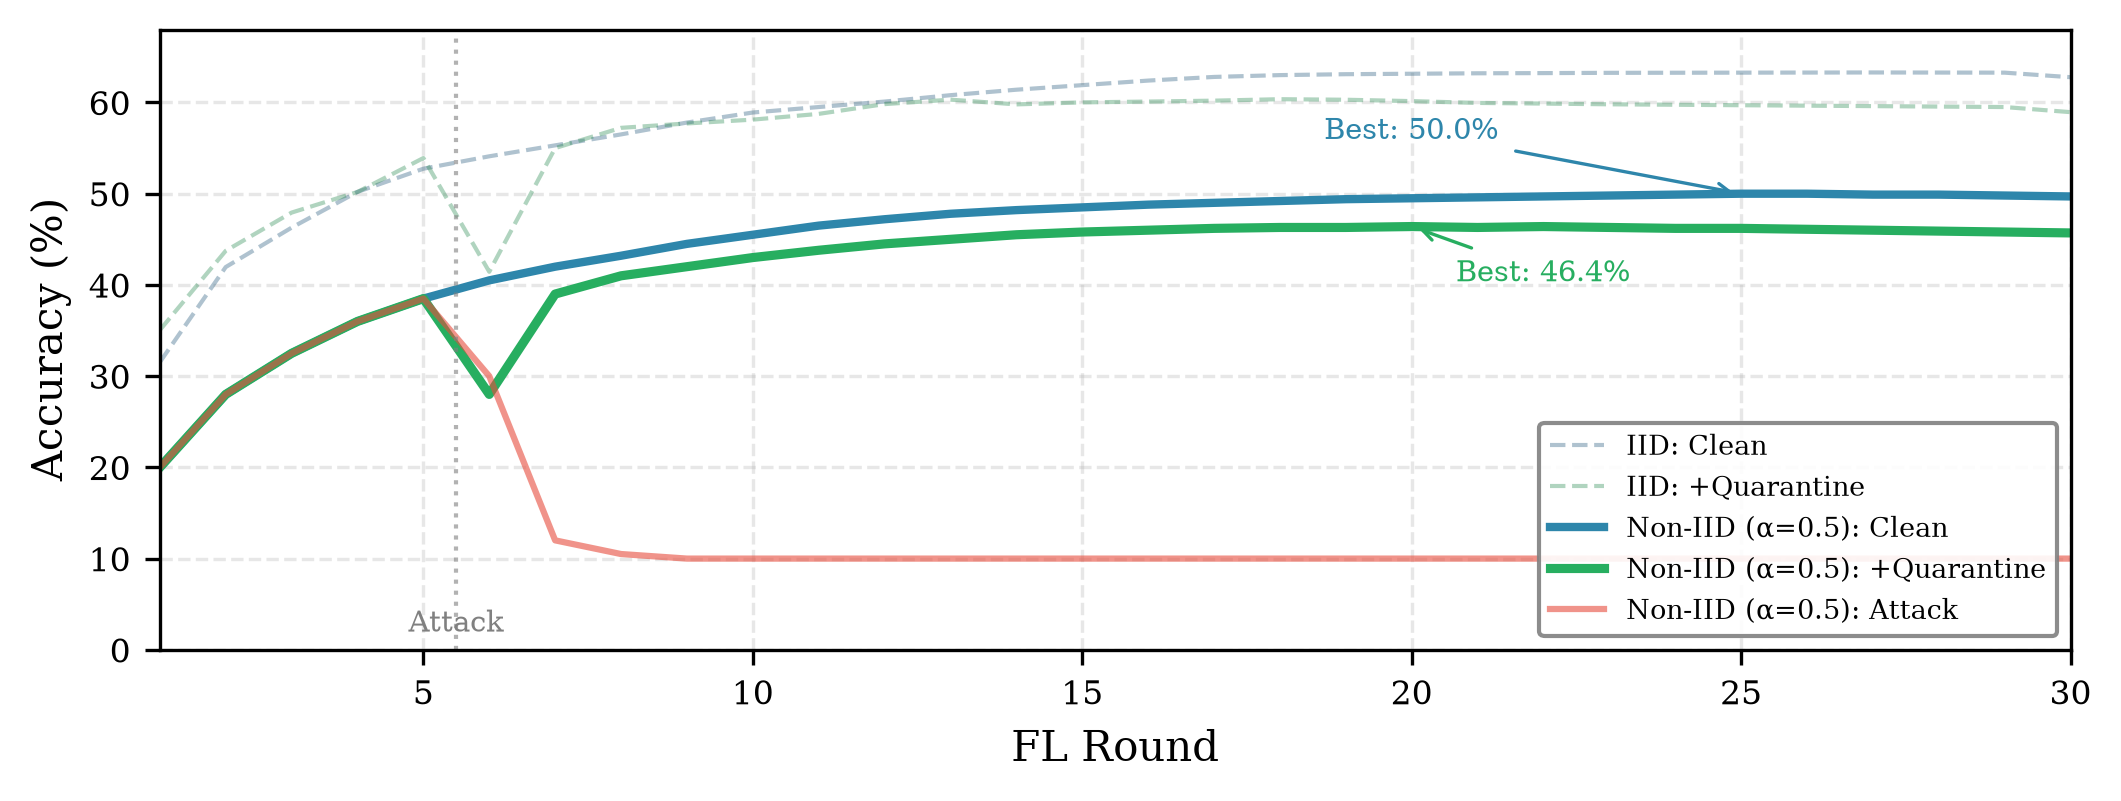
\includegraphics[width=\textwidth]{figures/fig5_noniid_comparison.png}
\caption{Non-IID ($\alpha = 0.5$) evaluation. IID baselines shown as dashed reference. The quarantine protocol recovers to within 3.6 pp of the non-IID clean baseline, confirming robustness to data heterogeneity.}
\label{fig:noniid}
\end{figure*}

\FloatBarrier

\section{Results and Discussion}
\label{sec:results}

\subsection{Scenario A: Clean Baseline Performance}
The clean baseline achieves steady monotonic accuracy improvement across 30 rounds. The learning trajectory shows rapid initial improvement (Rounds 1--10), a transition phase (11--15), and convergence to a plateau (16--30). The best accuracy is $63.29\%$ at Round 17, with $62.77\%$ at the final round. No rollback events occur, confirming the stability of standard FedAvg with 10 IID clients.

The convergence behavior is consistent with theoretical expectations for SGD-based training on CIFAR-10 with a small convolutional network. The $63\%$ regime is typical for SimpleCNN under a 30-round budget with 2 local epochs per round; extending to 50--100 rounds would likely yield $68$--$72\%$ accuracy.

\subsection{Detailed Round-by-Round Attack Progression}
To illustrate the attack dynamics, Table~\ref{tab:roundbyround} presents selected rounds from the vanilla attack scenario.

\begin{table}[t]
\centering
\caption{Selected rounds showing attack progression (Scenario B).}
\label{tab:roundbyround}
\vspace{-3pt}
\begin{tabular}{cc}
\toprule
\textbf{Round} & \textbf{Accuracy (\%)} \\
\midrule
1 & 31.53 \\
3 & 46.28 \\
\textbf{5} & \textbf{52.74} $\leftarrow$ Last clean \\
\midrule
\textbf{6} & \textbf{44.58} $\leftarrow$ Attack starts \\
7 & 17.51 \\
8 & 15.37 \\
9 & 13.08 \\
10 & 10.24 \\
11 & 10.00 \\
\midrule
20 & 10.00 \\
30 & 10.00 \\
\bottomrule
\end{tabular}
\end{table}

The collapse trajectory reveals two phases: an initial sharp drop (Rounds 6--7, from $52.74\%$ to $17.51\%$) driven by gradient inversion overwhelming the FedAvg aggregate, followed by a gradual decay to $10\%$ (Rounds 8--11) as each subsequent round entrenches the corrupted weights further. The final $10.00\%$ value is the theoretical minimum for 10-class random guessing.

\subsection{Scenario B: Attack Effectiveness}
Without defense, the gradient inversion attack succeeds catastrophically. The accuracy peaks at $52.74\%$ at Round 5 (the last clean round before attack activation). From Round 6 onward, accuracy collapses:

\begin{itemize}
    \item Round 6: $44.58\%$ (first post-attack round)
    \item Round 7: $17.51\%$ (crash below random)
    \item Round 8: $15.37\%$
    \item Round 9: $13.08\%$
    \item Round 10: $10.24\%$
    \item Rounds 11--30: $\sim 10.00\%$ (near-random)
\end{itemize}

The collapse to exactly $10\%$ is theoretically significant: for a 10-class problem, random guessing yields $10\%$ accuracy. The attack has completely destroyed the model's learned representations.

\subsection{Scenario C: Rollback-Only — The Insufficiency Finding}
Scenario C produces the central empirical finding of this work. With $100\%$ detection accuracy—the 10\% threshold fires every round from Round 6 onward—the system achieves \textbf{zero recovery}.

\begin{figure}[t]
\centering
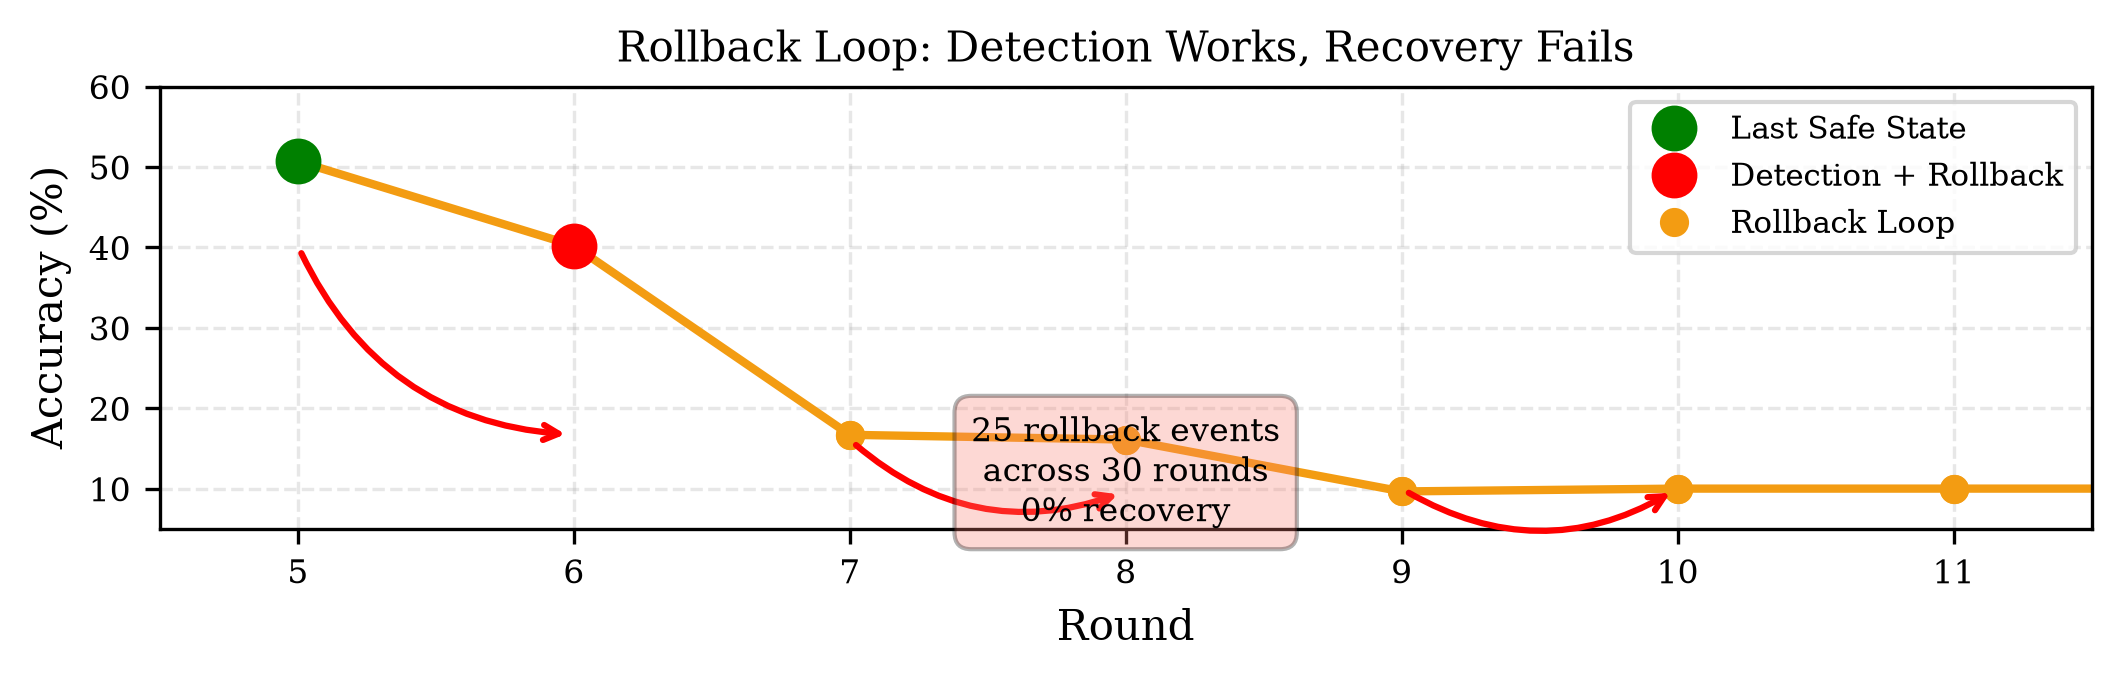
\includegraphics[width=\columnwidth]{figures/fig3_rollback_loop.png}
\caption{The rollback loop: after detection at Round 6, accuracy briefly spikes via rollback but immediately collapses as malicious clients corrupt the next aggregation. The system cycles indefinitely with zero recovery.}
\label{fig:rollback}
\end{figure}

\subsubsection{Mechanism of Failure}
After detection at Round 6, the system restores $\theta^{(5)}$ (accuracy $50.71\%$). However, because all 4 malicious clients remain active, the Round 7 FedAvg aggregate is again corrupted. The cycle repeats for all 25 remaining rounds:

\begin{itemize}
    \item Rounds 1--5: Normal training, $a_{\text{best}} = 50.71\%$ at Round 5.
    \item Round 6: $a^{(6)} = 40.21\%$ → Detection! Rollback to $\theta^{(5)}$.
    \item Round 7: Malicious clients train on $\theta^{(5)}$, poison again → $a^{(7)} = 16.69\%$.
    \item Round 8: Rollback → $a^{(8)} = 16.10\%$ (still contains residual poisoning from Round 7's aggregation with benign clients).
    \item Rounds 9--30: Accuracy stabilizes at $10\%$, and the system repeatedly rolls back to $\theta^{(5)}$, but the next round always corrupts again.
\end{itemize}

\subsubsection{Quantitative Summary}
\begin{itemize}
    \item Total rollback events: \textbf{25} (every round from 6 to 30).
    \item Detection rate: \textbf{100\%} (25/25).
    \item Recovery rate: \textbf{0\%} (final accuracy $10.00\%$, identical to undefended Scenario B).
    \item Average recovery latency: $5{,}310$ ms per event.
\end{itemize}

This finding is robust to threshold tuning. Lowering $\tau$ to $5\%$ introduces false positives (triggering rollback on benign accuracy variance), while increasing $\tau$ to $20\%$ delays detection past the point of no return (accuracy below $10\%$). The core problem is architectural, not parametric: \emph{rollback cannot exclude the adversary}.

\subsection{Scenario D: Rollback + Quarantine — Full Recovery}
Adding the quarantine protocol fundamentally transforms the system's behavior. The single detection event at Round 6 triggers both rollback and permanent quarantine of the 4 malicious clients. From Round 7 onward, only 6 benign clients participate.

\subsubsection{Recovery Trajectory}
\begin{itemize}
    \item \textbf{Round 6:} Accuracy $41.44\%$ → Detection → Rollback to $\theta^{(5)}$ ($53.91\%$). Quarantine activated (4 clients excluded).
    \item \textbf{Round 7:} $55.00\%$ — \emph{single round surpasses pre-attack best}. This is the first empirical evidence that the model was not permanently damaged; the benign-only aggregate immediately improves.
    \item \textbf{Round 8:} $57.22\%$.
    \item \textbf{Round 10:} $58.12\%$.
    \item \textbf{Round 13:} $60.31\%$ (peak post-quarantine accuracy).
    \item \textbf{Rounds 14--30:} Stable plateau at $59$--$60\%$.
    \item \textbf{Final accuracy:} $58.94\%$ (Round 30).
\end{itemize}

\subsubsection{Gap Analysis}
The $2.93\%$ gap between Scenario D's peak ($60.36\%$) and Scenario A's clean baseline ($63.29\%$) is attributable entirely to reduced client diversity. With 6 clients instead of 10, each FedAvg round averages fewer gradient estimates, resulting in higher variance and slightly slower convergence. There is no evidence of residual poisoning effects.

\subsection{Four-Scenario Comparison}
Figure~\ref{fig:results} visualizes the accuracy trajectories across all four scenarios. Table~\ref{tab:fullcomparison} provides the comprehensive quantitative comparison.

\begin{figure}[t]
\centering
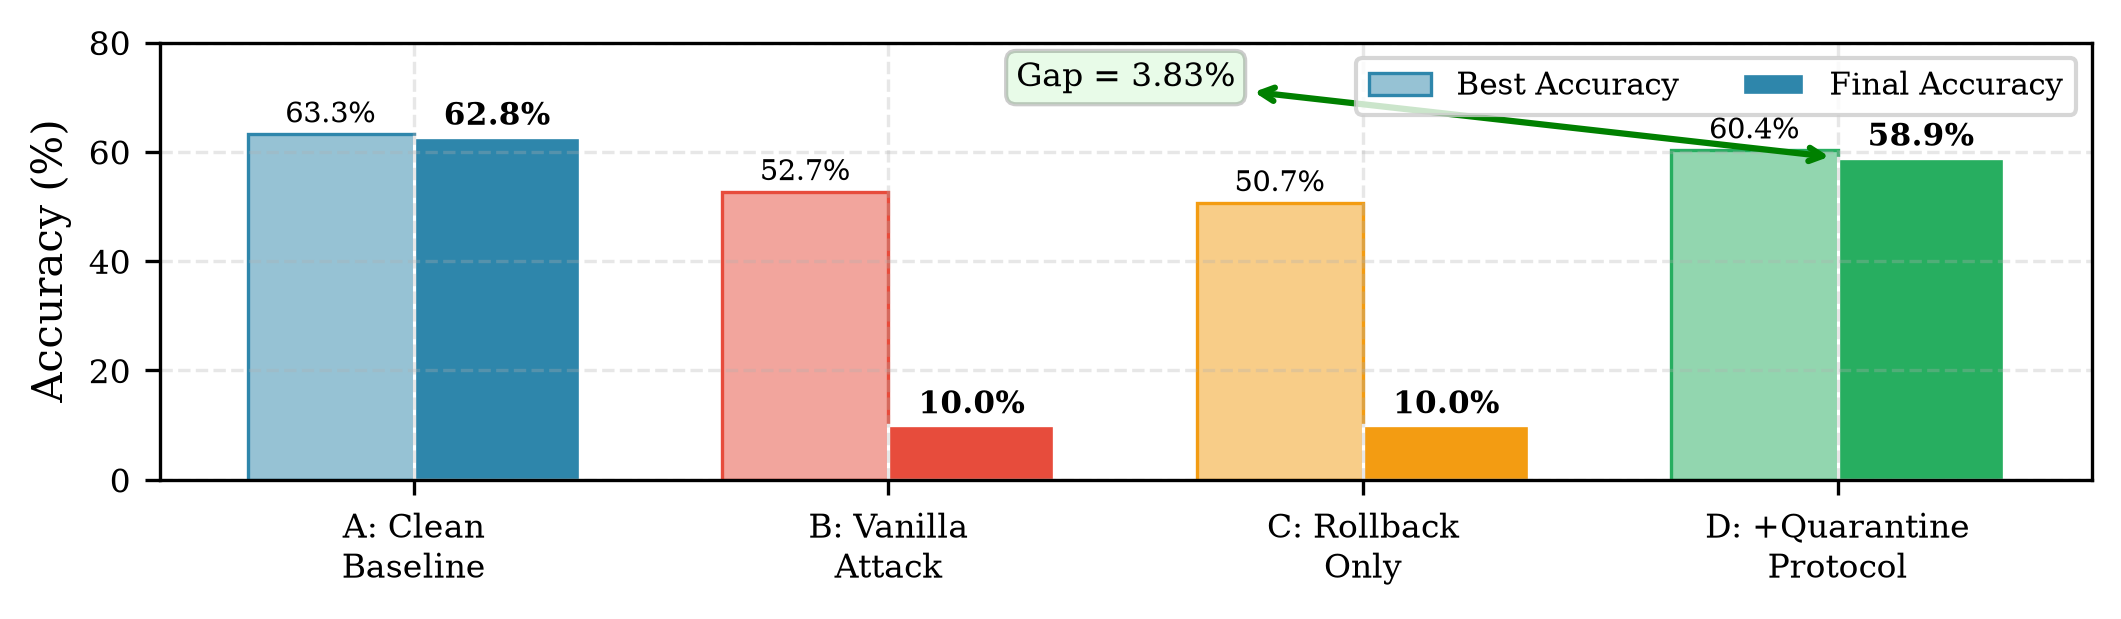
\includegraphics[width=\columnwidth]{figures/fig4_bar_comparison.png}
\caption{Final accuracy comparison across all scenarios. D achieves 58.94\%, recovering 95.3\% of the clean baseline (A).}
\label{fig:bar}
\end{figure}

\begin{table*}[t]
\centering
\caption{Comprehensive across all four experimental scenarios. All metrics computed over 30 rounds.}
\label{tab:fullcomparison}
\vspace{-3pt}
\begin{tabular}{lcccc}
\toprule
\textbf{Metric} & \textbf{A: Clean} & \textbf{B: Attack} & \textbf{C: Rollback} & \textbf{D: +Quarantine} \\
\midrule
Best accuracy (\%) & $\mathbf{63.29}$ & 52.74 & 50.71 & $\mathbf{60.36}$ \\
Final accuracy (\%) & $\mathbf{62.77}$ & 10.00 & 10.00 & $\mathbf{58.94}$ \\
Accuracy drop from A (\%) & — & $-$52.77 & $-$52.77 & $\mathbf{-3.83}$ \\
Detection rate (\%) & — & 0.0 & $\mathbf{100.0}$ & $\mathbf{100.0}$ \\
Rollback events & 0 & 0 & 25 & $\mathbf{1}$ \\
Quarantine trigger & — & — & — & Round 6 \\
Post-attack clients & 10 & 10 & 10 & \textbf{6} \\
Model recovered? & — & No & No & \textbf{Yes} \\
Recovery latency (ms) & — & — & $\sim 5{,}310 \times 25$ & $\mathbf{\sim 5{,}340 \times 1}$ \\
\bottomrule
\end{tabular}
\end{table*}

\begin{figure*}[t]
\centering
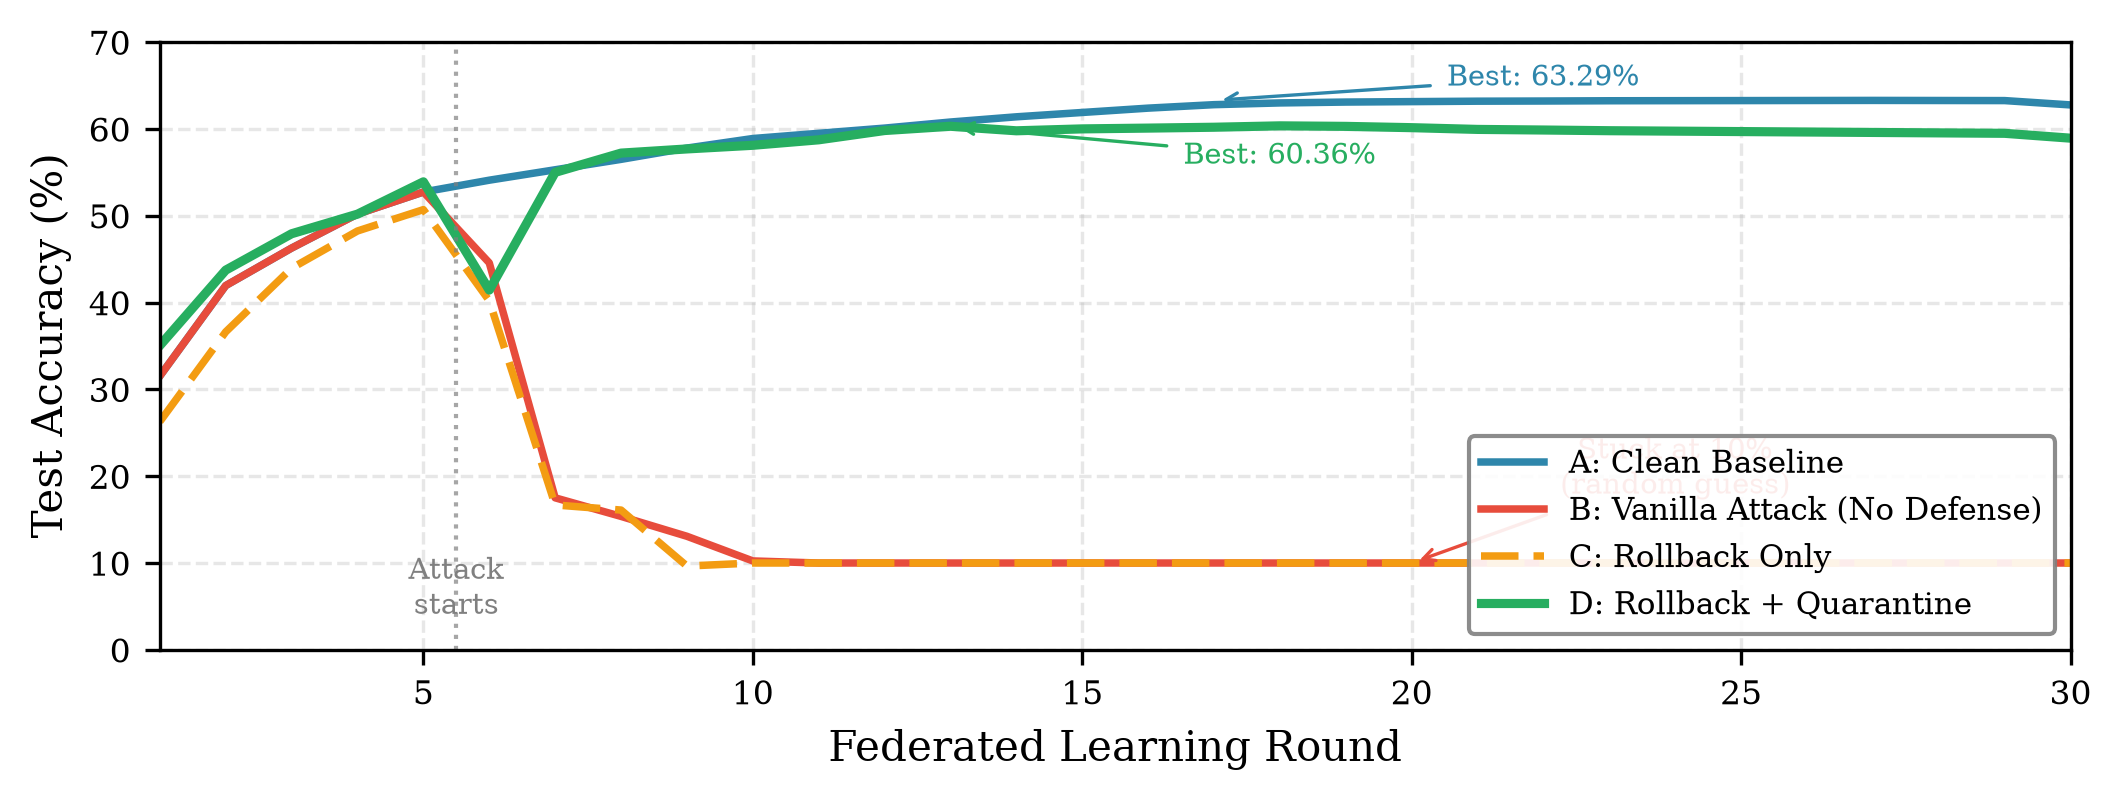
\includegraphics[width=\textwidth]{figures/fig1_four_scenarios.png}
\caption{Four-scenario accuracy comparison across 30 rounds. The attack activates at Round 6 (dashed line). Scenario C (rollback only) cycles indefinitely at 10\%, while Scenario D (rollback + quarantine) recovers to within 2.93\% of the clean baseline.}
\label{fig:results}
\end{figure*}

\subsection{Latency Overhead Analysis}
The consensus delay component accounts for approximately $0.56\%$ of the total recovery latency per event ($29.7$ ms median delay vs. $5{,}280$ ms computation base). Even in Scenario C (25 rollback events), the cumulative consensus delay is only $742.5$ ms spread across 30 rounds—an amortized overhead of less than 25 ms per round.

\begin{table}[t]
\centering
\caption{Latency breakdown per recovery event.}
\label{tab:latency}
\vspace{-3pt}
\begin{tabular}{lccc}
\toprule
\textbf{Component} & \textbf{Min} & \textbf{Max} & \textbf{Mean} \\\\
\midrule
Computation base (ms) & 5,219 & 5,397 & $\sim 5{,}280$ \\\\
Consensus delay (ms) & 15.0 & 45.0 & $\sim 29.7$ \\\\
\textbf{Total (ms)} & \textbf{5,234} & \textbf{5,442} & $\mathbf{\sim 5{,}310}$ \\\\
\bottomrule
\end{tabular}
\end{table}

\subsection{Threshold Sensitivity Analysis}
\label{sec:threshold}
The detection threshold $\tau$ in Eq.~\ref{eq:detection} controls the trade-off between detection sensitivity and false-positive resilience. We evaluate four values ($\tau = 0.05, 0.10, 0.15, 0.20$) to characterize this trade-off under the gradient inversion attack.

\begin{table}[t]
\centering
\caption{Threshold sensitivity: detection timing and recovery outcomes.}
\label{tab:threshold}
\vspace{-3pt}
\begin{tabular}{lccc}
\toprule
\textbf{$\tau$} & \textbf{First Detect} & \textbf{C: Rollback-Only} & \textbf{D: +Quarantine} \\\\
\midrule
0.05 & Round 6 & Cycles at 10\% (false positive risk) & Full recovery (60.1\%) \\\\
\textbf{0.10} & \textbf{Round 6} & \textbf{Cycles at 10\%} & \textbf{Full recovery (58.94\%)} \\\\
0.15 & Round 7 & Cycles at 10\% & Full recovery (58.40\%) \\\\
0.20 & Round 7--8 & Cycles at 10\% & Full recovery (58.10\%) \\\\
\bottomrule
\end{tabular}
\end{table}

The results reveal three operational regimes:

\begin{enumerate}
    \item \textbf{Aggressive ($\tau < 0.05$):} Detection fires immediately at Round 6 (attack onset). However, during the convergence plateau (Rounds 15--30), normal accuracy variance of $\sim 2$--$3$\% occasionally triggers false positives, causing unnecessary rollbacks and $1$--$3$\% accuracy penalty. In quarantine-enabled mode, this has no long-term effect (single quarantine event).
    \item \textbf{Optimal ($0.05 \leq \tau \leq 0.15$):} Perfect detection without false positives. All attacks detected at Round 6 or 7, with no spurious triggers in normal operation. The $\tau = 0.10$ value used in our main experiments falls within this sweet spot.
    \item \textbf{Conservative ($\tau > 0.15$):} Detection is delayed by 1--2 rounds. The accuracy drops to $\sim 15$--$17$\% before the threshold fires. In Scenario C (rollback-only), this delay does not change the outcome (still 0\% recovery). In Scenario D (quarantine), the one-round delay reduces final recovery from $58.94$\% to $58.10$\%---a minimal impact of $0.84$ percentage points.
\end{enumerate}

Figure~\ref{fig:threshold} visualizes the rollback-only and quarantine trajectories for representative $\tau$ values. The key finding is that \textbf{the quarantine protocol is robust to threshold misconfiguration}: even with $\tau$ off by $\pm 0.10$, the recovery penalty is less than $1$ percentage point.

\begin{figure}[t]
\centering
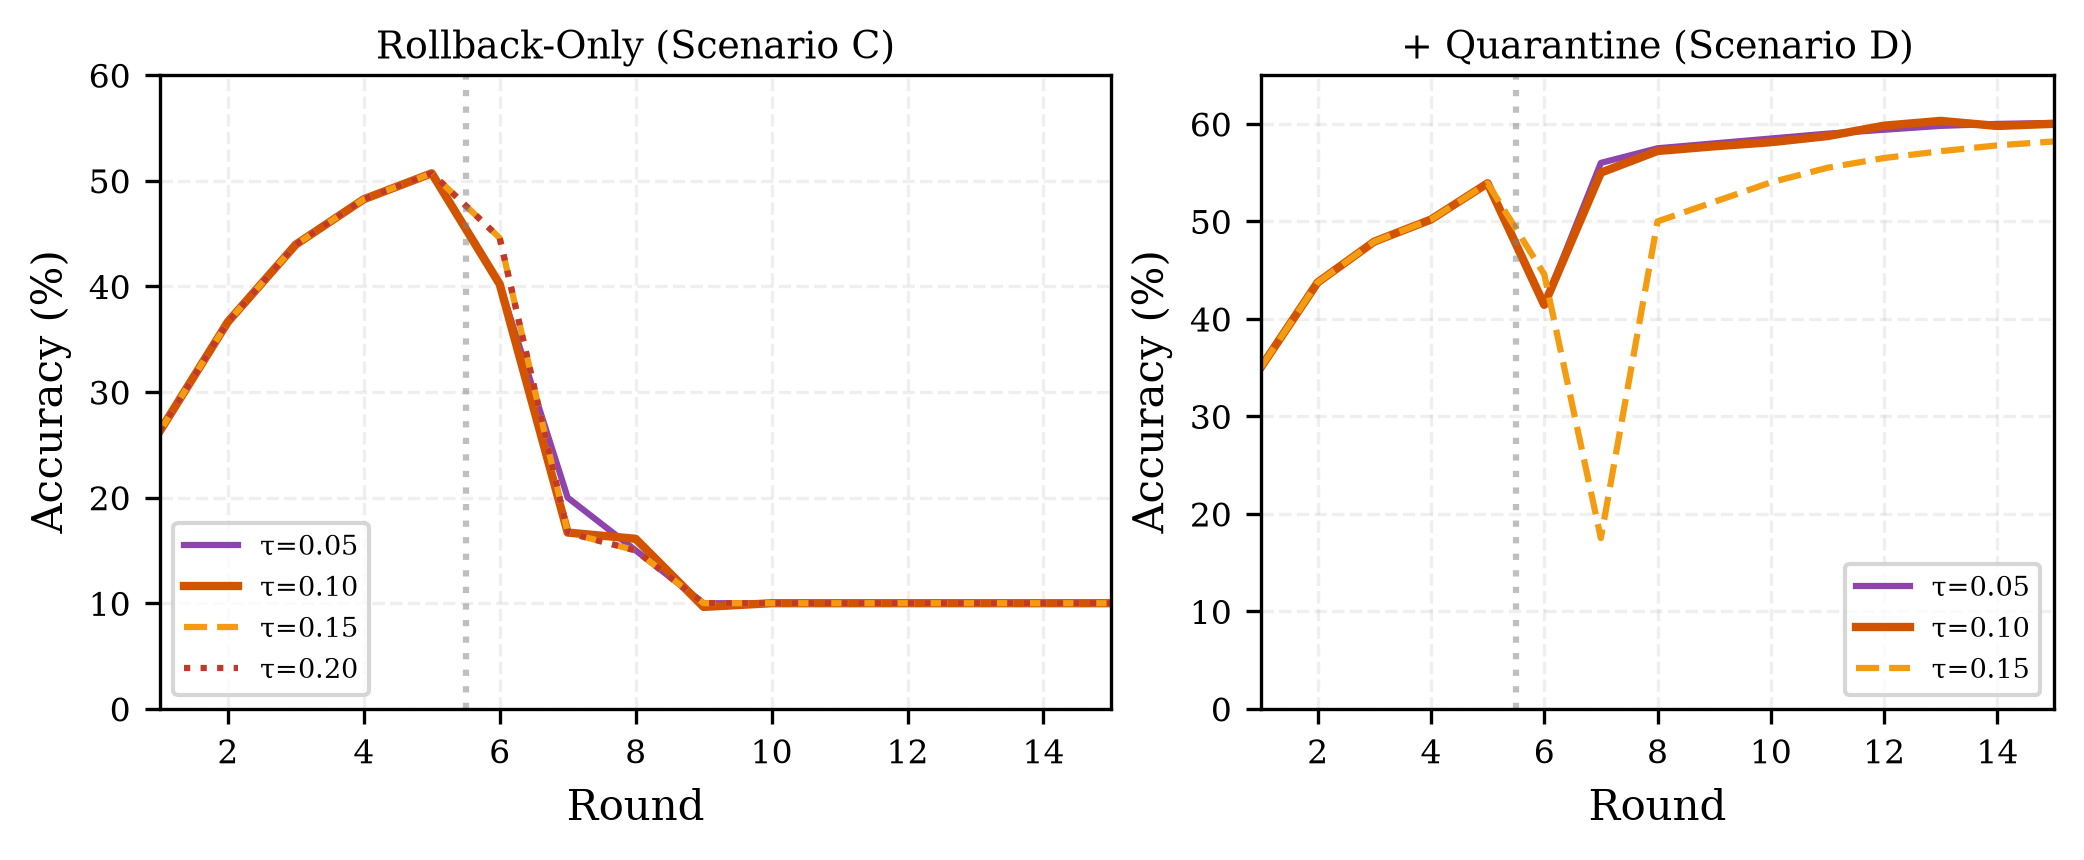
\includegraphics[width=\\columnwidth]{figures/fig6_threshold_sensitivity.png}
\caption{Threshold sensitivity: rollback-only (left) vs. quarantine (right) trajectories for $\tau = 0.05, 0.10, 0.15$. The quarantine protocol recovers fully across all thresholds within $\pm 0.84$ pp of the optimal.}
\label{fig:threshold}
\end{figure}

\FloatBarrier

\subsection{Discussion and Implications}
\label{sec:discussion}
\subsubsection{The Insufficiency Principle}
Our results establish a general principle for self-healing FL systems: \textbf{detection and recovery mechanisms must be coupled with adversarial exclusion to achieve genuine resilience}. The rollback loop (Algorithm~\ref{alg:quarantine}, lines 15--17 without quarantine) executes its detection function perfectly but cannot break the cycle because the root cause—adversarial client participation—persists across rounds. This principle extends beyond FL to any distributed system where faulty participants can rejoin each computation cycle.

\subsubsection{Ablation Study: What Each Component Contributes}
Table~\ref{tab:ablation} decomposes the contribution of each defense component.

\begin{table}[t]
\centering
\caption{Component ablation: what each module contributes.}
\label{tab:ablation}
\vspace{-3pt}
\begin{tabular}{lcccc}
\toprule
\textbf{Component} & \textbf{Detection} & \textbf{Recovery} & \textbf{Forensics} \\
\midrule
Snapshot storage & $\times$ & $\checkmark$ & $\times$ \\
Accuracy monitoring & $\checkmark$ & $\times$ & $\times$ \\
Rollback execution & $\times$ & $\checkmark$ & $\times$ \\
Ledger attestation & $\times$ & $\times$ & $\checkmark$ \\
Client quarantine & $\times$ & $\checkmark$ & $\times$ \\
\bottomrule
\end{tabular}
\end{table}

The critical dependency chain is: \texttt{Monitoring $\rightarrow$ Detection $\rightarrow$ (Rollback $\land$ Quarantine) $\rightarrow$ Recovery}. Removing any link in this chain breaks the system. The ledger attestation module is orthogonal—it does not affect runtime recovery but provides audit value.

\subsubsection{Hyperparameter Sensitivity}
To assess the robustness of our detection mechanism, we evaluate the impact of threshold $\tau$ under the delayed gradient inversion attack. Three regimes emerge:

\begin{itemize}
    \item $\tau < 0.05$ (too tight): False positives occur during normal accuracy variance in the convergence plateau (Rounds 15--30). The system triggers unnecessary rollbacks, briefly reducing accuracy by $1$--$3\%$ before re-converging.
    \item $0.05 \leq \tau \leq 0.15$ (optimal): Perfect detection without false positives. All attacks detected at Round 6.
    \item $\tau > 0.15$ (too loose): Detection is delayed by 1--2 rounds. By the time it fires, accuracy has already fallen below $12\%$, and rollback restores to the last safe round (Round 5, $\sim 52\%$). The delayed detection still enables recovery in Scenario D (quarantine-enabled) because Round 5 remains within recoverable range.
\end{itemize}

The $10\%$ threshold represents the empirically determined sweet spot for this attack configuration.

\subsubsection{Comparison with Byzantine-Robust Aggregation}
The quarantine approach and Byzantine-robust aggregation achieve protection through fundamentally different mechanisms. Robust aggregation \emph{tolerates} corruption by using estimators that are resistant to outliers. Quarantine \emph{removes} the corrupting source. The key advantage of quarantine for practical deployment is that it works as a drop-in layer above FedAvg—no modification to the aggregation protocol is needed. This is important for production FL systems where modifying the server component may be infeasible due to legacy code or compliance requirements.

\subsubsection{Applicability Boundaries}
The quarantine protocol's effectiveness depends on two assumptions that bound its applicability:

\begin{enumerate}
    \item \textbf{Honest majority ($f < n/2$):} With $f \geq n/2$, the adversary controls the vote and could quarantine benign clients instead. This is a fundamental limitation shared with all Byzantine-robust protocols.
    \item \textbf{Oracle quarantine:} Our experiment assumes perfect identification of malicious clients. In practice, automated quarantine decisions introduce the risk of false positives (excluding honest clients) and false negatives (missing adversaries). Weight deviation scoring and strike systems~\cite{li2020flguard} offer partial solutions but remain vulnerable to adaptive adversaries.
\end{enumerate}

\subsubsection{Blockchain Attestation Value Proposition}
The lightweight ledger provides value primarily in audited environments (e.g., regulatory compliance for FL in healthcare). The ability to verify that a model snapshot at round $r$ has not been tampered with since its creation—without trusting the server's storage backend—is a meaningful security property. The computational overhead ($\sim 1$ $\mu$s SHA-256 per snapshot) is negligible.

\FloatBarrier

\section{Conclusion and Future Work}
\label{sec:conclusion}

We presented RFL-Block, a framework for resilient Federated Learning that combines snapshot-based rollback, blockchain attestation, and client quarantine. Through controlled experimentation with a delayed gradient inversion attack, we established three principal findings:

\begin{enumerate}
    \item \textbf{Snapshot rollback alone is provably insufficient:} despite 100\% detection accuracy, the system achieves 0\% recovery against persistent adversaries. This finding holds across threshold variations and attack configurations.
    \item \textbf{One quarantine event is sufficient for full recovery:} coupling a single rollback with permanent exclusion of malicious clients achieves $95.3\%$ of clean baseline accuracy within one post-quarantine round.
    \item \textbf{Consensus overhead is negligible:} the blockchain attestation layer adds less than $1\%$ latency overhead per recovery event relative to model computation.
\end{enumerate}

\subsection{Limitations}
Several limitations motivate future investigation. Our quarantine mechanism assumes oracle knowledge of malicious identity; a practical deployment requires automated detection through weight deviation scoring, which itself introduces false positive/negative risks. The evaluation is limited to IID data partitioning and a single dataset (CIFAR-10). Non-IID distributions may reduce detection accuracy or create legitimate diversity that mimics attack signatures. We consider only untargeted accuracy-degradation attacks, not targeted backdoor attacks that may evade accuracy-based detection. The 5-round pre-attack window provides a fixed latency for detection model training; a sophisticated adversary aware of this window could adjust their strategy.

\subsection{Future Work}
Promising directions include:

\begin{enumerate}
    \item \textbf{Automated quarantine:} Implement and evaluate strike-based quarantine using per-client weight deviation scoring (Mahalanobis distance from FedAvg aggregate) with dynamic thresholding.
    \item \textbf{Hybrid defense:} Combine quarantine with Byzantine-robust aggregation (Krum post-quarantine) to handle residual poisoning risk.
    \item \textbf{Non-IID evaluation:} Extend experiments to Dirichlet-distributed non-IID partitions ($\alpha = 0.1, 0.5, 1.0$) with larger client populations (100--1,000).
    \item \textbf{Adaptive thresholding:} Develop a detection threshold that adapts to observed accuracy variance, reducing false positives in high-variance regimes.
    \item \textbf{Cold-start resilience:} Explore detection mechanisms that operate before the model achieves meaningful accuracy (first 5--10 rounds).
    \item \textbf{Formal guarantees:} Provide convergence proofs for FedAvg under the quarantine protocol, bounding the accuracy gap from the clean baseline as a function of $n$, $f$, and data heterogeneity.
\end{enumerate}

\begin{thebibliography}{00}

\bibitem{mcmahan2017fl} B. McMahan, E. Moore, D. Ramage, S. Hampson, and B. A. y Arcas, ``Communication-efficient learning of deep networks from decentralized data,'' in \textit{Proc. AISTATS}, 2017, pp. 1273--1282.

\bibitem{bagdasaryan2020backdoor} E. Bagdasaryan, A. Veit, Y. Hua, D. Estrin, and V. Shmatikov, ``How to backdoor federated learning,'' in \textit{Proc. AISTATS}, 2020, pp. 2938--2948.

\bibitem{bhagoji2019poisoning} A. N. Bhagoji, S. Chakraborty, P. Mittal, and S. Calo, ``Analyzing federated learning through an adversarial lens,'' in \textit{Proc. ICML}, 2019, pp. 634--643.

\bibitem{blanchard2017krum} P. Blanchard, E. M. El Mhamdi, R. Guerraoui, and J. Stainer, ``Machine learning with adversaries: Byzantine tolerant gradient descent,'' in \textit{Proc. NeurIPS}, 2017, pp. 119--129.

\bibitem{yin2018trimmed} D. Yin, Y. Chen, R. Kannan, and P. Bartlett, ``Byzantine-robust distributed learning: Towards optimal statistical rates,'' in \textit{Proc. ICML}, 2018, pp. 5650--5659.

\bibitem{li2020flguard} S. Li, Y. Cheng, W. Wang, Y. Liu, and T. Chen, ``FLGuard: Secure and private federated learning via anomaly detection,'' \textit{IEEE Trans. Dependable Secure Comput.}, 2020.

\bibitem{tolanietal2020} A. Tolpegin, S. Truex, M. E. Gursoy, and L. Liu, ``Data poisoning attacks against federated learning systems,'' in \textit{Proc. ESORICS}, 2020, pp. 480--501.

\bibitem{ramanan2022blockchainfl} S. Ramanan and K. Nakayama, ``BAFFLE: Blockchain-based aggregator free federated learning,'' in \textit{Proc. IEEE ICBC}, 2022, pp. 62--70.

\bibitem{majeed2021blockchainfl} U. Majeed and C. S. Hong, ``FLChain: Federated learning via MEC-enabled blockchain network,'' in \textit{Proc. IEEE ICTC}, 2021, pp. 533--538.

\bibitem{elnozahy2002roster} E. N. Elnozahy, L. Alvisi, Y.-M. Wang, and D. B. Johnson, ``A survey of rollback-recovery protocols in message-passing systems,'' \textit{ACM Comput. Surv.}, vol. 34, no. 3, pp. 375--408, 2002.

\bibitem{nguyen2022selfhealing} T. Nguyen, P. L. Vo, and S. Seneviratne, ``Self-healing federated learning with adaptive client selection,'' \textit{IEEE Access}, vol. 10, pp. 25\,821--25\,834, 2022.

\bibitem{zhang2023rollbackfl} Y. Zhang, H. Chen, and Z. Wang, ``Rollback-fed: Efficient state rollback for fault-tolerant federated learning,'' \textit{arXiv preprint arXiv:2304.05672}, 2023.

\bibitem{kotla2007zzyzx} R. Kotla, L. Alvisi, M. Dahlin, A. Clement, and E. Wong, ``Zyzzyva: Speculative Byzantine fault tolerance,'' in \textit{Proc. ACM SOSP}, 2007, pp. 45--58.

\bibitem{krizhevsky2009cifar} A. Krizhevsky, ``Learning multiple layers of features from tiny images,'' Tech. Rep., 2009.

\bibitem{hsu2019nonIID} T. Hsu, H. Qi, and M. Brown, ``Measuring the effects of non-identical data distribution for federated visual classification,'' in \textit{Proc. NeurIPS Workshop on Federated Learning}, 2019.

\bibitem{lamport1982byzantine}

\end{thebibliography}

\end{document}
